\section{Understanding Shortcut-Stacked-Encoder}\label{sec:understanding}
In this section we give analyse the sentence representations of Shortcut-Stacked Encoder\textsuperscript{$\dagger$} by visualizing how they encode (Section §\ref{sec:insights_sent_repr}) and leverage (Section §\ref{sec:insights_sent_alignment}) information from natural language text, coming from \ac{SNLI}. Additionally we show experiments, underlining the presented insights.
\subsection{Motivation}
The major downside of neural networks is the lack of interpretability \citep{goldberg2017Apr}, thus their capabilities on a lower level can only be estimated by finding meaningful evidence for their failures or sucesses on the task at hand. While analysing errors may lead to conclusions \textit{what} does not work, \textit{why} it does not work is in many cases left to intuition. Other machine-leanring classes like probabilistic or symbolic techniques do not suffer from this problem, leading to an increasing interest in visualization techniques for neural networks. Most visualitations of sentence-representations to date focus on attention-based approaches showing how words are aligned to each other such as by \cite{shen2018reinforced} or \cite{im2017distance}. To the best of our knowledge, no insights have been gained to understand the final sentence representation in vector space. In this section we demonstrate how this representation, arising from max-pooling, can be interpreted, using the Shortcut-Stacked Encoder\textsuperscript{$\dagger$} as the model to analyze. Intuitively, understanding how the Shortcut-Stacked Encoder\textsuperscript{$\dagger$} encodes information can be helpful for the task at hand of improving it using external resources. 
\newline

\noindent
While we did not manage to leverage the insights gained in this chapter to increase the performance, it might be helpful for future work.
NN nicht gut interpretierbar

\subsection{Insights on the sentence representation}\label{sec:insights_sent_repr}
In this section we show how we analyse the informaation that is present within the sentence representions, what kind of information is encoded and demonstrate, that the sentence representation can manually be adjusted in a meaningful way.
\subsubsection{Approach}
We use Shortcut-Stacked Encoder\textsuperscript{$\dagger$}, trained on \ac{SNLI}, for our analyses. This model creates for input each sentence $x$, cosnisting of words, represented as $x_i$, a sentence representation $r \in \mathbb{R}^{2048}$ with $r_j$ being the $j$th dimension of $r$. Arising from $x$, $r$ captures the relevant information for the task at hand and is used in many neural networks without a deeper understanding what each $r_j$ actually encodes. We shed light into the dimensionewise meaning of the sentence represnetation by identifying which word is responsible for the actual value of $r_j$. 
\paragraph*{Method}\label{sec:understanding1_method}
For simplicity, We explain our applied method and the reason why we use Shortcut-Stacked Encoder using a more general neural architecture of \ac{LSTM}s, a simple uni-directional \ac{RNN}.
Figure \ref{fig:rnn} (left) shows the recursive workflow of such a \ac{RNN}, following the notations of \cite{goldberg2017Apr}.
\begin{figure}[tph!]
\centering
	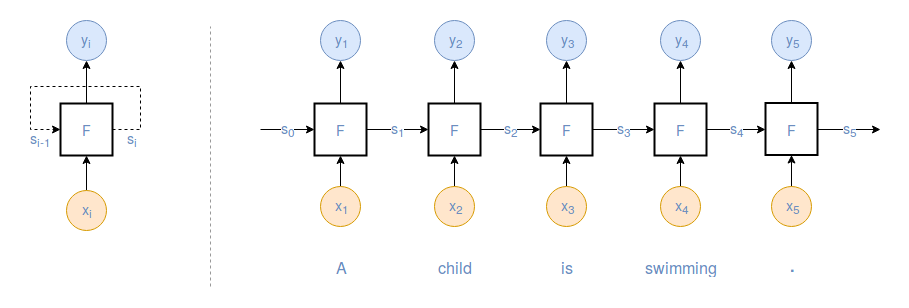
\includegraphics[totalheight=5.5cm]{fig/rnn.png}
	\caption{General architecture of a \ac{RNN} (left). Example sentence in an unrolled \ac{RNN} (right).}
	\label{fig:rnn}
\end{figure}
Maintaining an internal state $s \in \mathbb{R}^m$, for $m$-dimensional representations, the network recursively iterates over the input sequence $x$, aggregating in each timestep the previous state $s_{i-1} \in \mathbb{R}^m$ with the current input $x_i$ using the function $F$. This state is then used for the next iteration and output via a mapping function as $y_i \in \mathbb{R}^m$. Multiple implementation variants exist of $F$ and what is shared across iterations. \ac{LSTM}s for instance use several neural gates to learn what information should be used, output or forgotten. This procedure ca be seen with an example sentence yb unrolling the network in Figure \ref{fig:rnn} (right). In typial setups a neural network may either choose to use $s_t$ or $y_t$ for a sequence length of $t$ as the final sentence representation \citep{goldberg2017Apr}, since the network iterated over the full input sequence and contains the relevent information, if optimized for it. Even though the architecture of different versions of \ac{RNN} may be well understood and has a logical meaning, the actual procedure of deriving concrete representations within a trained model is hard to understand. We leverage the fact that the Shortcurt Stacked Encoder uses max-pooling over all $y_i$ to gather the sentence representation rather than using $y_t$ or $s_t$ by identifying what $y_t$ has the highest value within a given dimension and mapping this dimension to the word $x_t$ of the input sentence. As an example consider the sentence in Figure \ref{fig:rnn} (right). For each timestep $t$ a new vector $y_t$ is produced. As done by \cite{nie2017shortcut} we concatenate all $y_t$ to a matrix $\mathbb{R}^{m \times t}$, with $m$ being the representation size and each vector $y_t$ being the $t$th row within $M$. Assuming a dimensionality of $m = 3$, an examplatory matrix $M$ for the given sentence ``A child is swimming .'' is displayed in Figure \ref{fig:example_process_understanding}. 
\begin{figure}[tph!]
\centering
	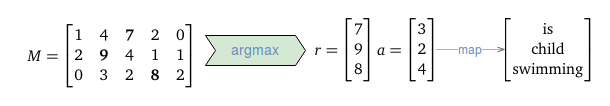
\includegraphics[totalheight=2cm]{fig/example_process_understanding.png}
	\caption{Visualized example of extracting interpretable information of the max-pooled seentence representations with a dimensionality of 3.}
	\label{fig:example_process_understanding}
\end{figure}
Additiobnally to creating the sentence representation $r$ by applying wor-wise max-pooling on $M$, we collect the vector $a$, containing the column indizes, that are responsible for the values within $r$. These can directly be mapped to the word of the source sentence and thus be interpreted by humans. It should be notted that due to the nature of the multi layer \ac{biLSTM} each $y_t$ does not only contain the word at $x_t$ but its context. While this somehow may lead to less accurate mapping, we found that the chosen method is sufficient to gain some meaningful insights on sentence encoding.

\paragraph*{Analysed data}
To reduce noise and aming for sentences that Shortcut-Stacked Encoder\textsuperscript{$\dagger$} seems to have a proper understanging about, we sample 1000 sentence representations from the \ac{SNLI} train data in the following strategy. We group all sentence pairs ($p$, $h$) sharing the same premise and only keep groups if all samples belonging to the same group are classified correctly. Thus, we reduce the amount of sentences that are definetly misunderstood by the model, that would be harder to interpret. For now we are not interested in the actual relation between $p$ and $h$ and therefore create a pool of the remaining sentences, by treating $p$ and $h$ equally and splitting their connections apart. After removing duplicate sentences, the most frequent sentence length for the remaining representations is 8. To reduce noise that may arise from different sentence lengths, we only consider sentences of a length of 8 and randomly sample 1000 sentence representations. All experiments in this chapter are based on the same instances, unless otherwise stated.
\newline

\noindent
In addition to the representation values each sample contains the following information:
\begin{itemize}
\item \textbf{Token:} The tokens that triggered the maximum value for the representation.
\item \textbf{Token position:} Positional information about the responsible tokens within the sentence.
\item \textbf{Lemma:} The lemmata of the responsible tokens.
\item \textbf{\ac{POS}:} The \ac{POS} tags of the responsible tokens.
\item \textbf{Dependency Parse:} The tags of the responsible tokens within the dependency parse tree.
\end{itemize}
Lemmatizing, \ac{POS}-Tagging and dependency parsing were conducted using spaCy.

\subsubsection{Detection of relevant dimensions}
manual research
identify relevant information
get understanding of the representation and how to interret it

create tool
label data and sort by label freqency + SD + dimension positions

responsible word i nitcht genug, value is immer wichtig
\subsubsection{Dimension-wise Analysis}
\paragraph{Positional information}
\paragraph{Semantic information}
\paragraph{Syntactic information}
\paragraph{Evaluation of the impact of female and male dimensions}
\subsubsection{Conclusion}
weg??
\subsection{Insights on the sentence alignment}\label{sec:insights_sent_alignment}
\subsubsection{Approach}
\subsubsection{Entailment analysis}
\subsubsection{Neutral and contradiction analysis}
\subsubsection{Experiments}
\subsubsection{Conclusion}
- eher experimental, need different models w maxpooling, mehr daten, mehr experiments, ...
\subsection{Errors of the base model}